%%%%%%%%%%%%%%%%%%%%%%%%%%%%%%%%%%%%%%%%%
% Beamer Presentation
% LaTeX Template
% Version 1.0 (10/11/12)
%
% This template has been downloaded from:
% http://www.LaTeXTemplates.com
%
% License:
% CC BY-NC-SA 3.0 (http://creativecommons.org/licenses/by-nc-sa/3.0/)
%
%%%%%%%%%%%%%%%%%%%%%%%%%%%%%%%%%%%%%%%%%

%----------------------------------------------------------------------------------------
%	PACKAGES AND THEMES
%----------------------------------------------------------------------------------------

\documentclass{beamer}

\mode<presentation> {

\usetheme{Madrid}
\usefonttheme{serif} 
\setbeamertemplate{navigation symbols}{}
}

\usepackage{graphicx} % Allows including images
\usepackage{booktabs} % Allows the use of \toprule, \midrule and \bottomrule in tables
\usepackage[T1]{fontenc}
\usepackage[utf8]{inputenc}
\usepackage{amsmath}
\usepackage{color}
\usepackage[czech]{babel}
\usepackage{lmodern}  
\usepackage{rotating}
\usepackage{scrextend}
\usepackage{pifont}
\usepackage{hyperref}
\usepackage{bm}

%----------------------------------------------------------------------------------------
%	TITLE PAGE
%----------------------------------------------------------------------------------------

\title[Block 1]{Praktikum z ekonometrie} % The short title appears at the bottom of every slide, the full title is only on the title page

\author{VŠE Praha} % Your name
\institute[4EK417] % Your institution as it will appear on the bottom of every slide, may be shorthand to save space
{
% Your institution for the title page
\medskip
\textit{Tomáš Formánek} % Your email address
}
\date{} % Date, can be changed to a custom date

\begin{document}

\begin{frame}
\titlepage % Print the title page as the first slide
\end{frame}

\begin{frame}
\frametitle{Block 1 -- Missing data -- Outline} % Table of contents slide, comment this block out to remove it
\tableofcontents % Throughout your presentation, if you choose to use \section{} and \subsection{} commands, these will automatically be printed on this slide as an overview of your presentation
\end{frame}

%----------------------------------------------------------------------------------------
%	PRESENTATION SLIDES
%---------------------------------------------------------------------------------------
\section{The nature of missing data}
\begin{frame}
\frametitle{The nature of missing data}

\begin{itemize}
  \item[] Missing completely at random (\textit{MCAR})
  \begin{itemize}
  \item The probability that an observation $X_i$ is missing is unrelated to the value of $X_i$ or to the value of any other variables.
  \item Any piece of data is equally likely to be missing.
  \item Analyses based on data with \textit{MCAR} observations remain unbiased. We may lose power (increased standard errors), but the estimated parameters are not biased by the absence of data.
  \end{itemize}
  \vspace{0.2cm}
  \item[] Missing at random (\textit{MAR})
  \begin{itemize}
  \item Data meets the requirement that missingness does not depend on the value of $X_i$ after controlling for another variable in our analysis.
  \item For example, data are MCAR in a specific (demographic) subgroup. 
  \end{itemize}
  \vspace{0.2cm}
  \item[] Missing Not at Random (\textit{MNAR})
  \begin{itemize}
  \item Missigness of $X_i$ depends on its value (e.g. income in surveys)
  \item The only way to obtain an unbiased estimates of (regression) parameters is to model the missingness.
  \end{itemize}
\end{itemize}


\end{frame}

%------------------------------------------------
\section{Traditional treatment of missing data}
\begin{frame}[fragile] % Need to use the fragile option when verbatim is used in the slide
\frametitle{Traditional treatment of missing data}


\textbf{Listwise deletion (complete cases analysis)}
\vspace{0.2cm}
  \begin{itemize}
  \item  We omit all rows with missing data – missing information for at least one variable in the $i$-th individual observation. Then, we run our analyses on the observations that remain. This often results in a substantial decrease in sample size. Under the assumption that data are missing completely at random, LRMs lead to unbiased parameter estimates – still, we lose power due to exclusion of (potentially large number of) observations.
  \end{itemize} 

\begin{block}{R code}
\begin{verbatim}
newData <- data[complete.cases(data)==T, ] 
# data is a data.frame
# or
newData <- na.omit(data) 
\end{verbatim}
\end{block}

\end{frame}

%------------------------------------------------

\begin{frame}
\frametitle{Traditional treatment of missing data}


\textbf{Hot deck imputation}
\vspace{0.2cm}
  \begin{itemize}
  \item  Historically used by the US Census Bureau (since 1950’s). Respondent’s missing data were replaced by observed replacement data – drawn at random from a group of similar participants. Suitable, given only a few missing observations need to be replaced and given the draw is random.
  \end{itemize} 

\end{frame}


%------------------------------------------------
\begin{frame}
\frametitle{Traditional treatment of missing data}
\textbf{Mean substitution}
\vspace{0.2cm}
  \begin{itemize}
  \item[\ding{51}] Simple
  \item[\ding{55}] In simple linear regression models (SLRMs), this adds no new information but increases sample size – that leads to underestimated standard errors only.
  \end{itemize} 
  \vspace{0.2cm}
\textbf{Example:} Data on salary and citation level of publications. 62 cases with complete data and 7 cases for which the citation index was missing. Correlations and regression coefficients were compared as follows:

\begin{table}
\begin{tabular}{l c c c c}
\toprule
Analysis & $n$ & $corr$ & $\widehat{\beta}_1$ & $\textit{s.e.}(\widehat{\beta}_1)$\\
\midrule
Complete cases only & 62 & .55 &  310.747 & 60.95 \\
With mean substitution & 69 & .54 &  310.747 & 59.12 \\
\bottomrule
\end{tabular}
\end{table}
\end{frame}
%------------------------------------------------
\begin{frame}
\frametitle{Traditional treatment of missing data}
\textbf{Mean substitution, contnd.} \\
\medskip
\begin{itemize}
    \item Mean imputation can be valid especially when data \\are missing as MCAR.
    \smallskip
    \item It is fast, simple, easy to implement, and no cases are excluded.
    \smallskip
    \item But even under MCAR, this method still leads to underestimation of the population variance. 
    \smallskip
    \item Bias (in variance estimation) is proportional to \\
    $( \textnormal{nobs} - 1)/( \textnormal{nobs} + \textnormal{nmis} - 1)$. \\Smaller standard errors increase the possibility of Type I errors.
\end{itemize}
\end{frame}
%------------------------------------------------
\begin{frame}
\frametitle{More advanced treatment of missing data}
\textbf{Regression substitution}
  \begin{itemize}
  \item Uses linear regression (auxiliary LRM) to predict what the missing values of regressors should be -- on the basis of other variables that are present.
  \item For SLRMs, the same problem of error variance as in mean substitution remains. We do not add more information but we increase the sample size and (spuriously) reduce the standard error.
  \item May be useful for MLRMs.
   \end{itemize}
  \vspace{0.2cm}
\textbf{Stochastic regression substitution}
  \begin{itemize}
  \item This approach adds a randomly sampled residual term from the normal (or other) distribution to each value estimated by regression substitution. Adding a bit of random error to each substitution reduces, but does not eliminate, the problem of spurious reduction of the standard errors.
   \end{itemize}
\end{frame}
%------------------------------------------------
\begin{frame}
\frametitle{More advanced treatment of missing data}

\textbf{Maximum Likelihood Expectation-Maximization}
  \begin{itemize}
  \item Computationally complex, maximum likelihood approach to the estimation of missing values Many approaches exist (e.g. the Expectation-Maximization algorithm)
  \item[] \scriptsize{\url{https://www.uvm.edu/~dhowell/StatPages/Missing_Data/Missing-Part-Two.html}}
   \end{itemize}
 
\end{frame}

%------------------------------------------------
\section{Modern Approaches to missing data}
\subsection{Multiple imputation for CS data}
\begin{frame}
\frametitle{Multiple imputation  for CS data}
\textbf{Multiple Imputation (MI) }\\
\texttt{R}: $\left\lbrace \texttt{mice}  \right\rbrace , \,\, \left\lbrace \texttt{mi}  \right\rbrace, \,\, \left\lbrace \texttt{Amelia}  \right\rbrace, \, $ \dots\\
  \vspace{0.5cm}
MI motivation and algorithm\\
  \vspace{0.2cm}
  \begin{itemize}
  \item Create several (say, 5) imputed values (versions) for each missing item -- regressor $x_{ij}$.
  \medskip
  \item Each of the (5) versions of imputed data is used for estimation \\(using OLS, ML or other adequate approach)
  \medskip
  \item Information obtained from all (e.g. 5) estimates is conveniently summarized.
 \end{itemize}
 \end{frame}
%------------------------------------------------
\begin{frame}
\frametitle{Multiple imputation (MI)}
Multiple imputation scheme (example with $m=3$ imputations):\\
\vspace{-1cm}
\begin{figure}
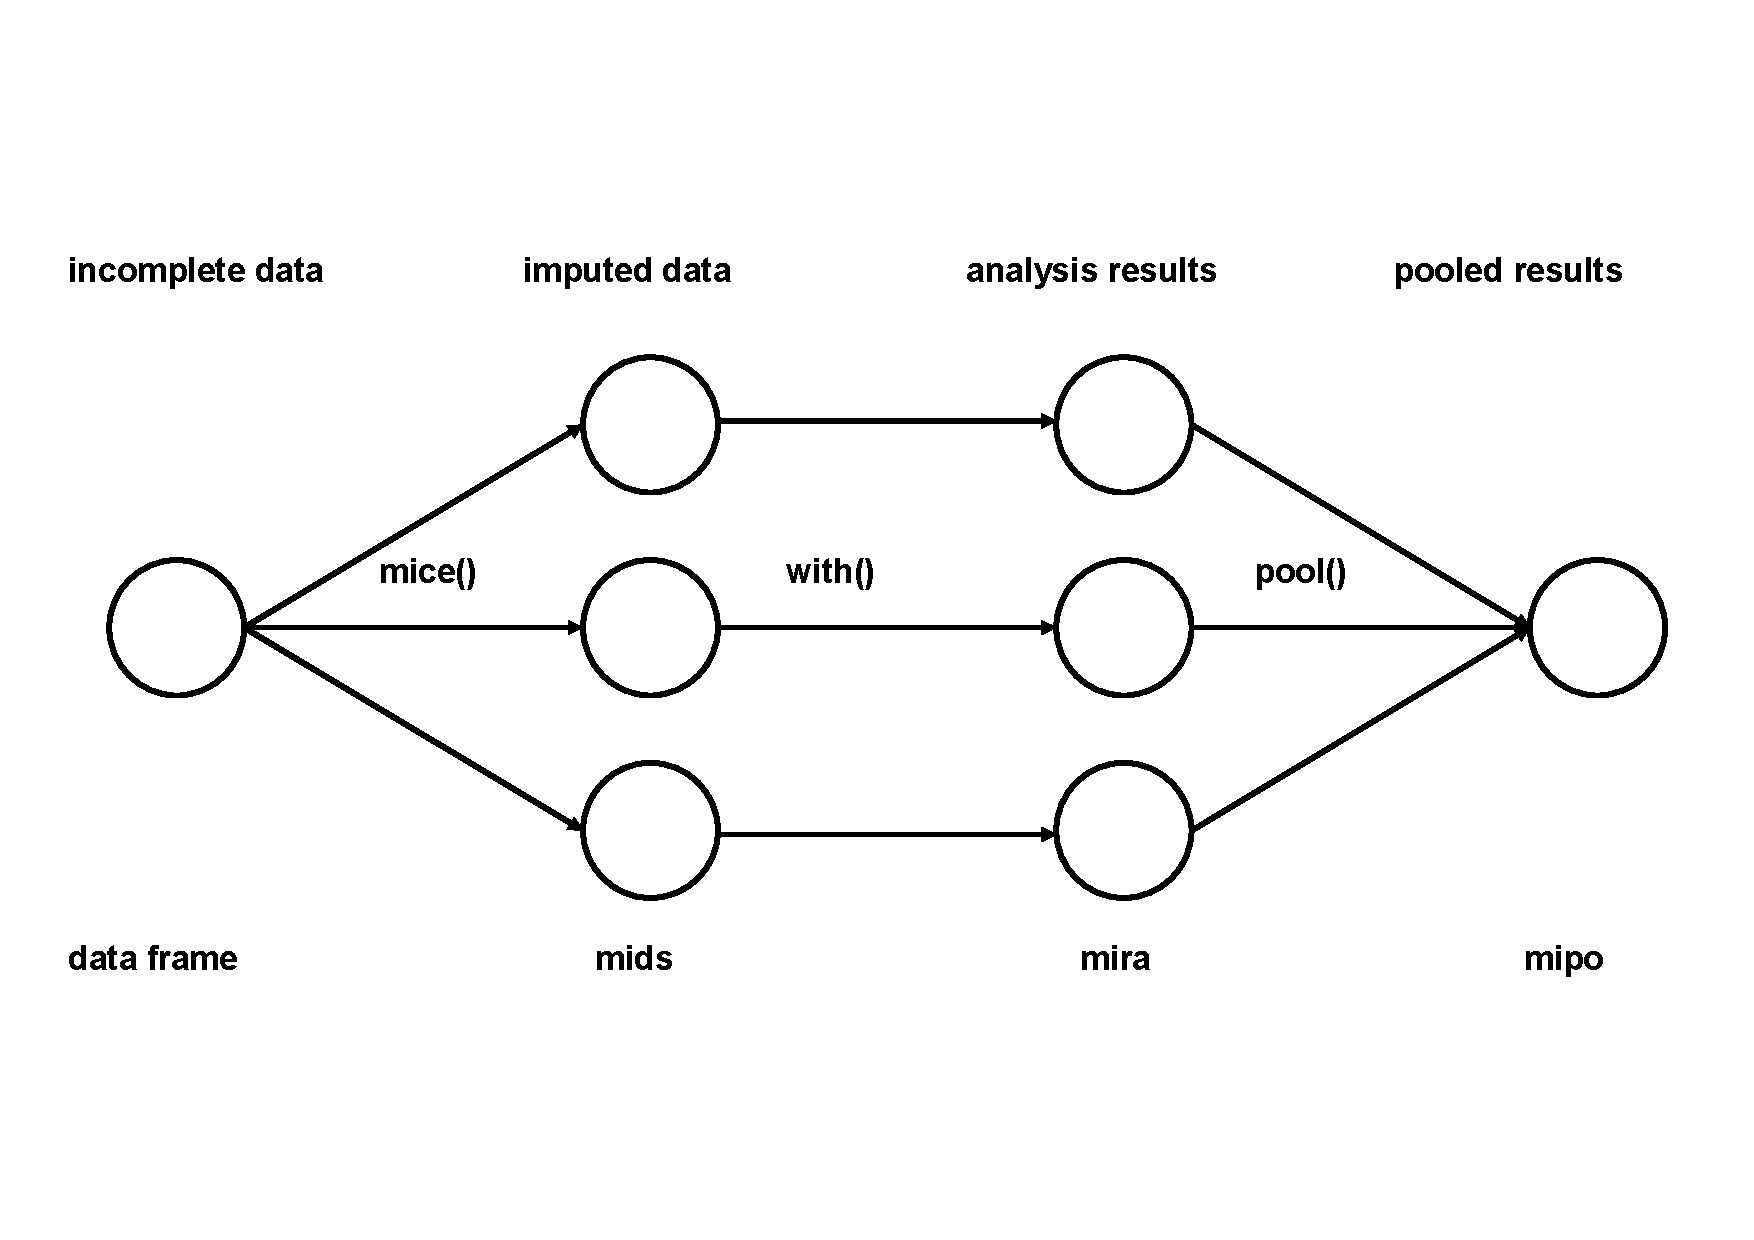
\includegraphics[width=1\linewidth]{IMG/mice_scheme.pdf}
\end{figure}
\centering
\vspace{-2.2cm}
$\left\lbrace \texttt{mice}  \right\rbrace$ object--types used for MI.
 \end{frame}
%------------------------------------------------
\begin{frame}
\frametitle{Multiple imputation (MI)}
\textbf{Multiple imputation - 7 choices to be made}\\
\smallskip
\begin{enumerate}
    \item Decide on MAR assumption plausibility (MAR/MNAR).
    \item Imputation model choice (univariate, multivariate, data type).
    \item Choice of predictors for MI.
    \item Should we impute variables that are functions of incomplete variables (e.g. interaction terms)?
    \item Choice of order of imputation (can affect results).
    \item MI is (generally) based on a numerical algorithm: we need to choose starting setup and control (limit) the number of iterations.
    \item We need to choose $m$ -- the number of imputed datasets.
\end{enumerate}
\smallskip
In \texttt{R} ($\{ \textnormal{mice} \}$), most of the choices have generally valid default setting.\\
\smallskip
However -- all the choices are always made in MI and they affect the resulting imputations.
\end{frame}
%------------------------------------------------
\begin{frame}
\frametitle{Multiple imputation (MI)}
\textbf{Predictive mean matching (\texttt{pmm}) in \texttt{R}} -- general description\\
\bigskip
\begin{itemize}
    \item Implemented in \{mice\} and other packages.
    \medskip
    \item General purpose semi-parametric imputation method.
    \medskip
    \item Suitable especially for imputing quantitative variables \\that are not normally distributed.
    \medskip
    \item Imputations are restricted to previously observed values.
    \medskip
    \item Can preserve non-linear relations even if the structural part \\of the imputation model is wrong.
\end{itemize}
\end{frame}
%------------------------------------------------
\begin{frame}
\frametitle{Multiple imputation (MI)}
\textbf{Predictive mean matching (\texttt{pmm}) in \texttt{R}} -- algorithm\\
\medskip
Suppose there is a single variable $x$ that has some cases with missing data, and a set of relevant variables $\bm{z}$ with no missing data:
$$
\{ x_i, \bm{z}_i\};~i = 1, \dots , n
$$
\vspace{-0.5cm}
\begin{enumerate}
    \item[1] For cases with no missing data, estimate LRM $x_i \leftarrow \bm{z}_i$, \\producing $\hat{\bm{\beta}}$ and $\textnormal{var}(\hat{\bm{\beta}})$ estimates.
    \medskip
    \item[2] Make a random draw from the ``posterior predictive distribution'' of $\hat{\bm{\beta}}$, producing a new set of coefficients $\hat{\bm{\beta}}^{\ast}$.\\
    \medskip
    \begin{itemize}
        \item Typically, this would be a random draw from a multivariate normal distribution with mean $\hat{\bm{\beta}}$ and cov. matrix $\textnormal{var}(\hat{\bm{\beta}})$. \\
    \medskip 
    \item This step is necessary to produce sufficient variability in the imputed values, and is common to all ``proper'' methods of MI.
    \end{itemize}
\end{enumerate}
\end{frame}
%------------------------------------------------
\begin{frame}
\frametitle{Multiple imputation (MI)}
\textbf{Predictive mean matching (\texttt{pmm}) in \texttt{R}} -- algorithm contnd.\\
\bigskip
\begin{enumerate}
    \item[3] Using ~$(\bm{z}_i \hat{\bm{\beta}}^{\ast})$~, generate predicted values $\hat{x}_i$ for \textbf{all cases}, \\both with data missing on $x_i$ and with data observations present.
    \medskip
    \item[4] For each case with missing $x_i$, identify a set of cases with observed $x_j$ values whose \textbf{predicted} $\hat{x}_j$ values are ``close'' to the predicted $\hat{x}_i$ values (missing data cases).
    \medskip
    \begin{itemize}
        \item For ``close'' values, proximity rules are defined separately.
    \end{itemize}
    \medskip
    \item[5] From among the close cases for each missing $x_i$, randomly choose one $x_j$ and use its observed value to substitute for the missing value.
    \medskip
    \item[6] In MI algorithm, repeat steps 2 through 5 for each of the $m$ imputed datasets.  
\end{enumerate}
\end{frame}
%------------------------------------------------
\begin{frame}
\frametitle{Multiple imputation (MI)}
\textbf{Predictive mean matching (\texttt{pmm}) in \texttt{R}} -- recap.\\
\medskip
\begin{itemize}
    \item Compared with regression-based methods, \texttt{pmm} produces imputed values that are much more like real values. 
    \smallskip
    \begin{itemize}
        \item If the original variable is skewed, imputed values will also be skewed.
        \smallskip
        \item If the original variable is bounded by 0 and 100, imputed values will also be bounded by 0 and 100.
        \smallskip
        \item If the real values are discrete (say, number of children), imputed values will also be discrete. 
    \end{itemize} 
    \smallskip
    \item Generally speaking,  there’s no mathematical proof/theory to justify \texttt{pmm}.
    \smallskip
    \item \texttt{pmm} efficiency can be demonstrated by Monte Carlo simulations.
\end{itemize}
\end{frame}
%------------------------------------------------
\begin{frame}
\frametitle{Multiple imputation (MI)}
\textbf{Multiple Imputation (empirical output example) }
\begin{figure}
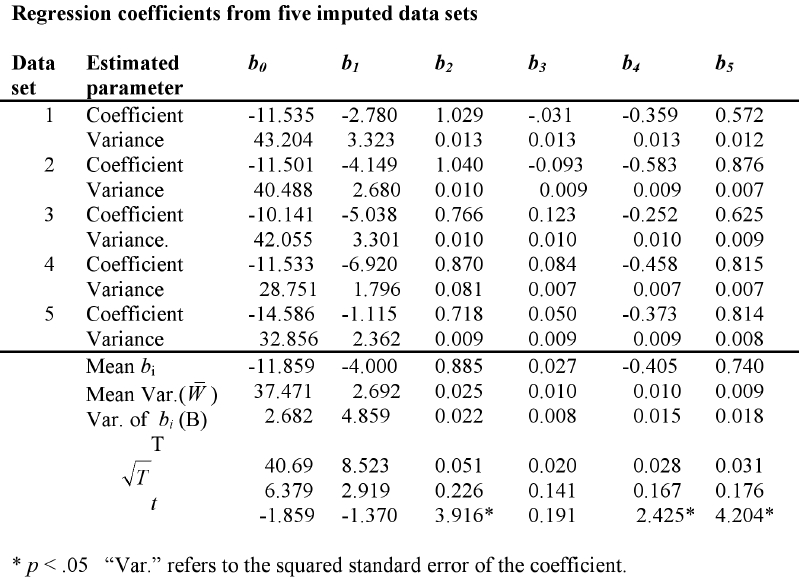
\includegraphics[width=0.7\linewidth]{IMG/mitable.jpg}
\end{figure}
\scriptsize{\url{https://www.uvm.edu/~dhowell/StatPages/Missing_Data/Missing-Part-Two.html}}
\end{frame}
%------------------------------------------------
\subsection{Multiple imputation for TS data}
\begin{frame}
\frametitle{Multiple imputation for TS data}

 \end{frame}
%------------------------------------------------

\section{Missing dependent variable data}
\begin{frame}
\frametitle{Missing dependent variable data}

\textbf{Special considerations apply to missing dependent variable data}

\begin{itemize}
  \item If we can assume that data are missing completely at random \textit{(MCAR)}, we will lose power because of smaller sample sizes, but we will not have problems with biased estimates.
  \item If data are missing not at random \textit{(MNAR)}, the \textbf{only way to obtain an unbiased estimate of parameters is to model missingness}. In other words we need to use a model that accounts for the missing data.
  \item Broadly speaking, such models are:
  \begin{itemize}
    \item Censored Regression Models (e.g. duration analysis) 
    \item Truncated Regression Models 
    \item Sample Selection Correction models (Heckit)
    \item \dots
  \end{itemize}
\end{itemize}

\end{frame}
%------------------------------------------------
\end{document}